\chapter{Badania}

Celem badań była ocena skuteczności wybranych algorytmów w rozwiązywaniu problemu przepływowego z przezbrojeniem. Obliczenia zostały przeprowadzone na zbiorze zadań z który składał sie następujących projektów:
\begin{enumerate}
	\item Liteboard.
	\item Chiliboard.
	\item Jetson Nano baseboard.
	\item KBox.
	\item HackRF One.
\end{enumerate}

\newpage
\section{Liteboard}

Liteboard jest to komputer jednopłytkowy (Single Board Computer) oparty na module liteSOM~\cite{liteboard}. Projekt ten posiada elementy elektroniczne i mechaniczne po obu stronach laminatu.

\breakparagraph{}
Ilość elementów elektronicznych: 178.

\begin{table}[H]
	\centering
	\caption{Poszczególne czasy na maszynach dla strony A}
	\begin{tabular}{lll}
		\toprule
		Nazwa maszyny                 & Czas operacji $[s]$ & Czas przezbrojenia $[s]$ \\
		\midrule
		stanowisko z sitodrukiem      & 10                  & 15                       \\
		automat pick\&place           & 540                 & 180                      \\
		ręczne układanie elementów & 15                  & 0                        \\
		lutowanie w piecu             & 300                 & 0                        \\
		lutowanie ręczne             & 85                  & 0                        \\
		kontrola wizualna             & 100                 & 0                        \\
		\bottomrule
	\end{tabular}
\end{table}

\begin{table}[H]
	\centering
	\caption{Poszczególne czasy na maszynach dla strony B}
	\begin{tabular}{lll}
		\toprule
		Nazwa maszyny                 & Czas operacji $[s]$ & Czas przezbrojenia $[s]$ \\
		\midrule
		stanowisko z sitodrukiem      & 0                   & 0                        \\
		automat pick\&place           & 0                   & 0                        \\
		ręczne układanie elementów & 0                   & 0                        \\
		lutowanie w piecu             & 0                   & 0                        \\
		lutowanie ręczne             & 80                  & 0                        \\
		kontrola wizualna             & 10                  & 0                        \\
		\bottomrule
	\end{tabular}
\end{table}

% \begin{figure}[H]
% 	\centering
% 	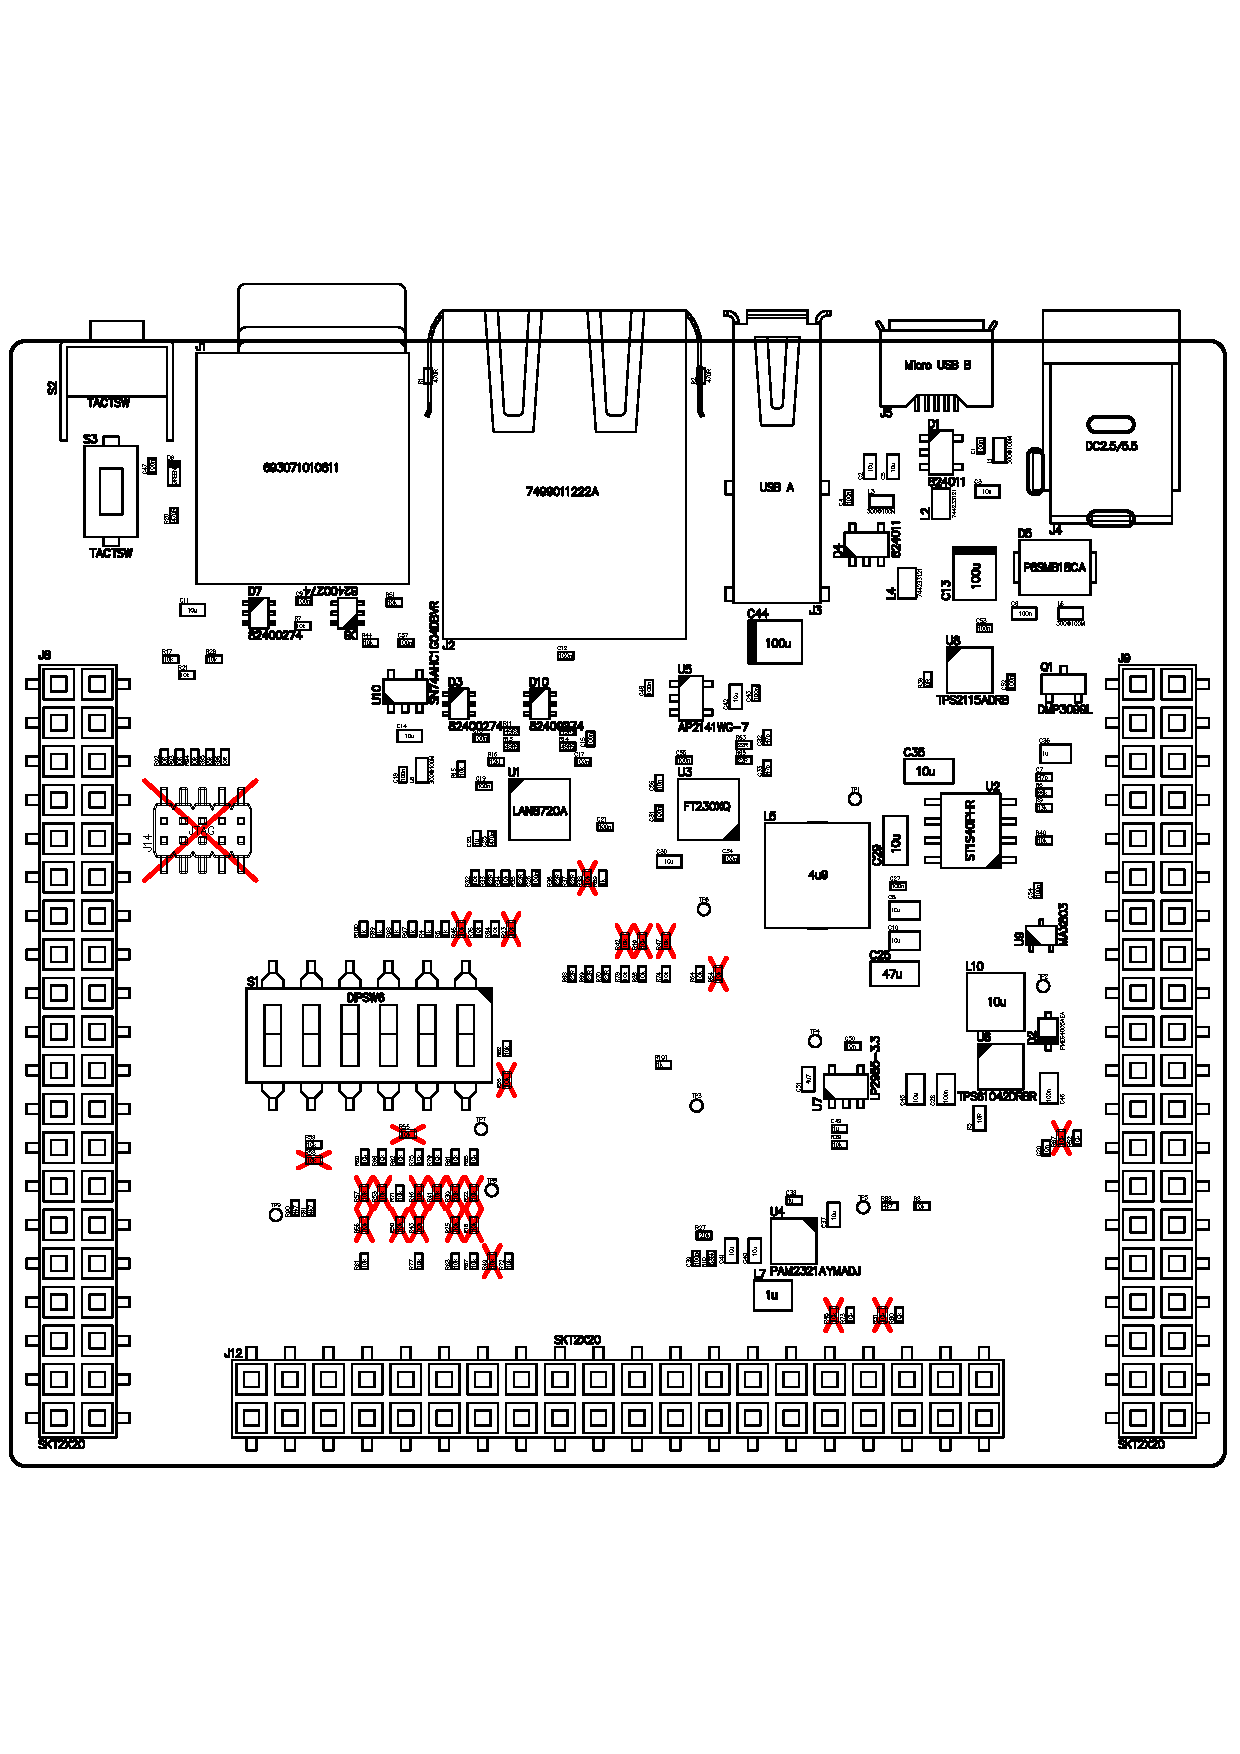
\includegraphics[scale=0.6,clip, trim=0cm 4cm 0cm 4cm]{./chapters/chapter5/liteboard_A.PDF}
% 	\caption{Jakaśnazwanato strona A}
% 	\label{baza_danych}
% \end{figure}

% \begin{figure}[H]
% 	\centering
% 	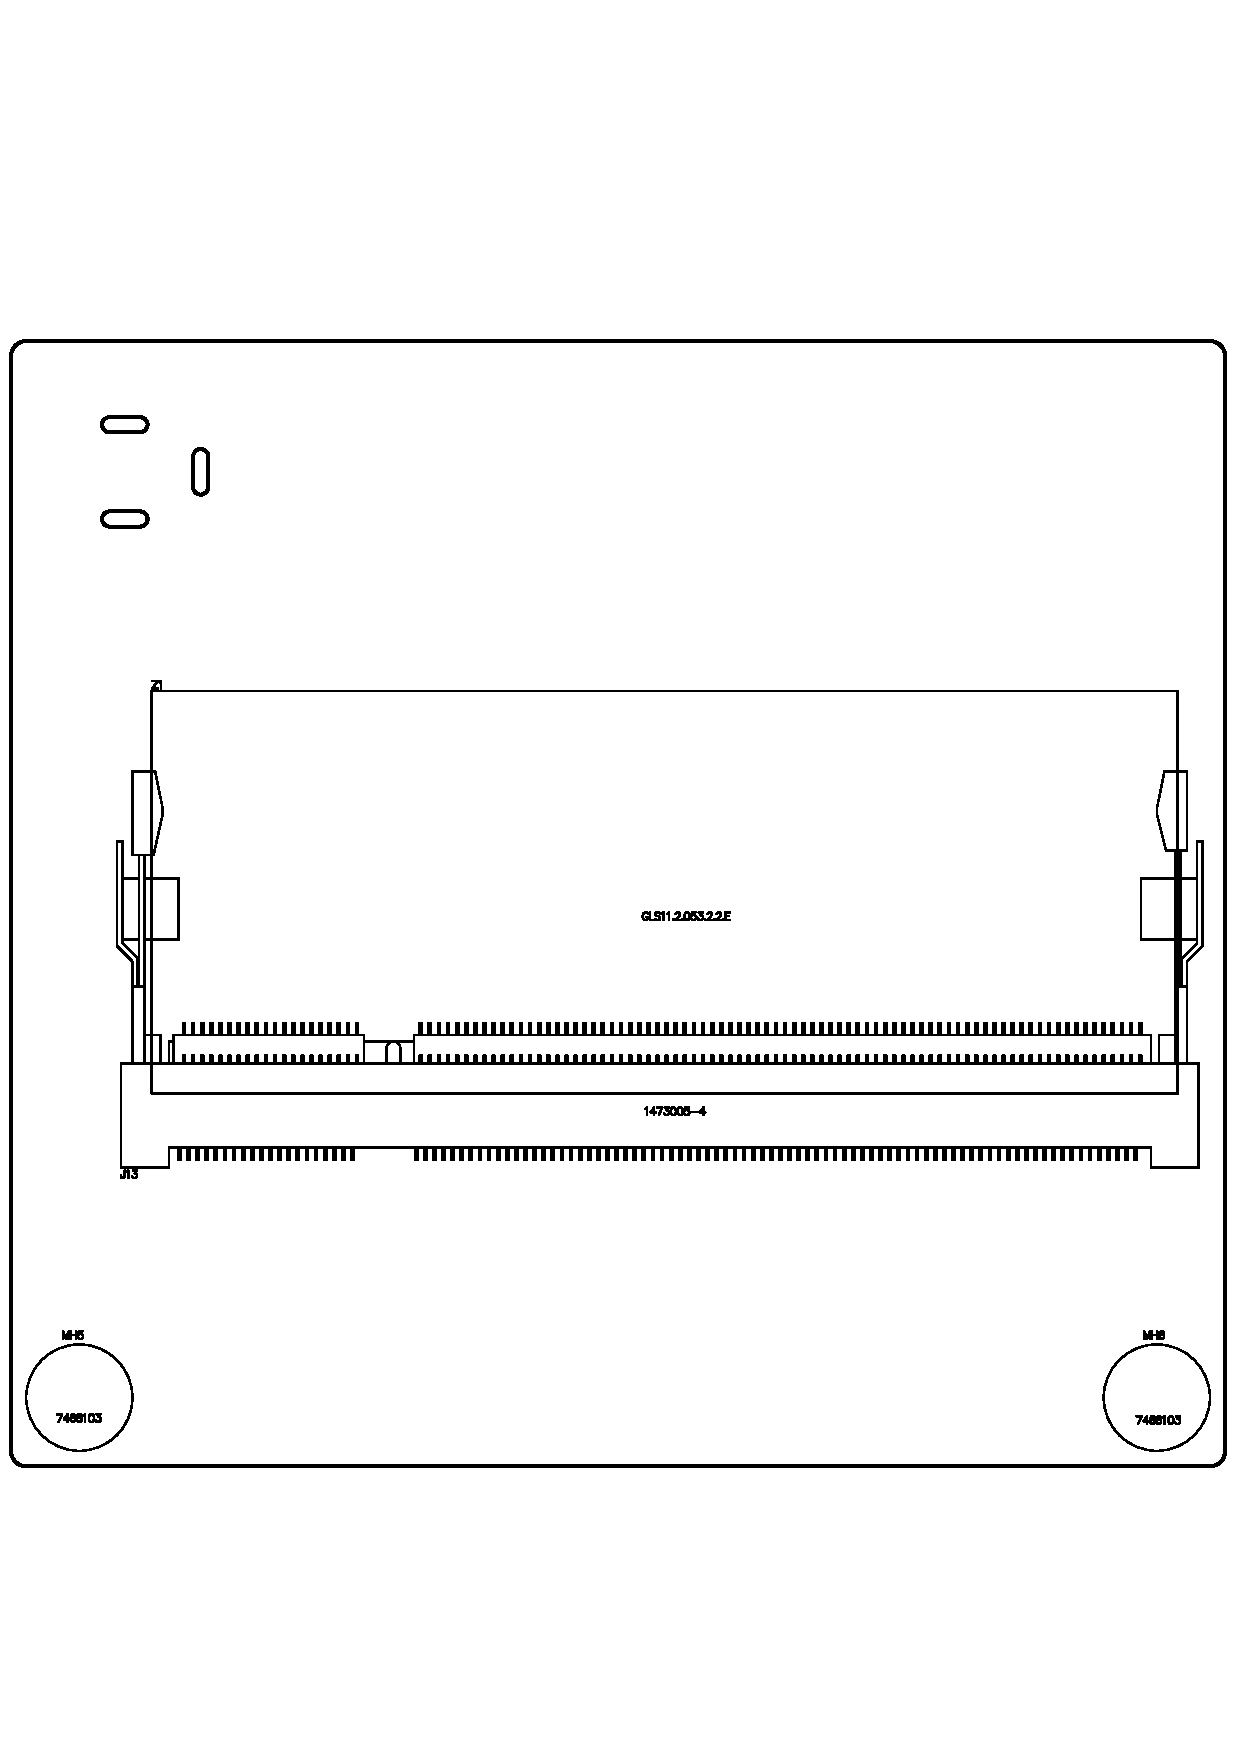
\includegraphics[scale=0.6,clip, trim=0cm 4cm 0cm 4cm]{./chapters/chapter5/liteboard_B.pdf}
% 	\caption{Jakaśnazwanato strona B}
% 	\label{baza_danych}
% \end{figure}

\begin{figure}[!htb]
	\begin{minipage}{0.5\textwidth}
		\centering
		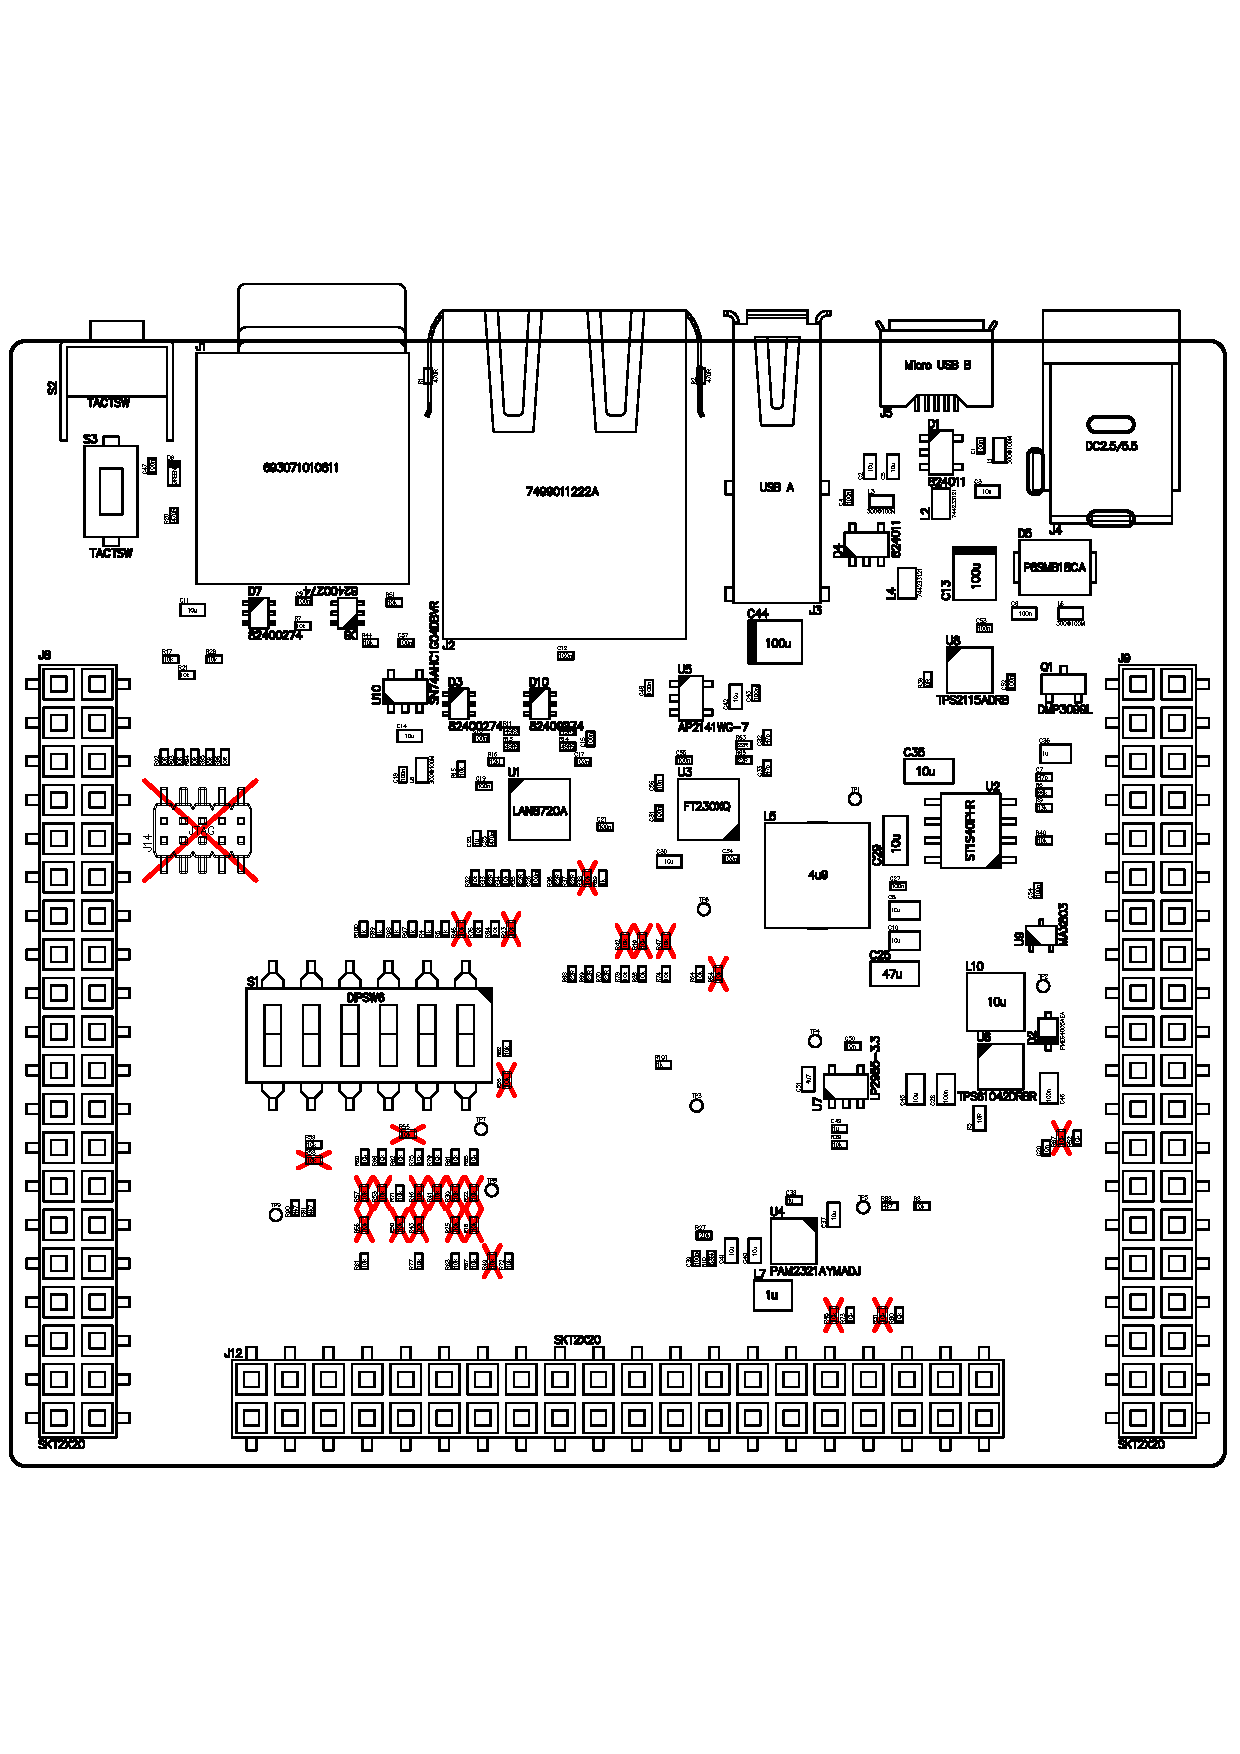
\includegraphics[width=0.9\linewidth,clip, trim=0cm 4cm 0cm 4cm]{./chapters/chapter5/liteboard_A.PDF}
		\caption{Strona A}\label{chilli:StronaA}
	\end{minipage}\hfill
	\begin{minipage}{0.5\textwidth}
		\centering
		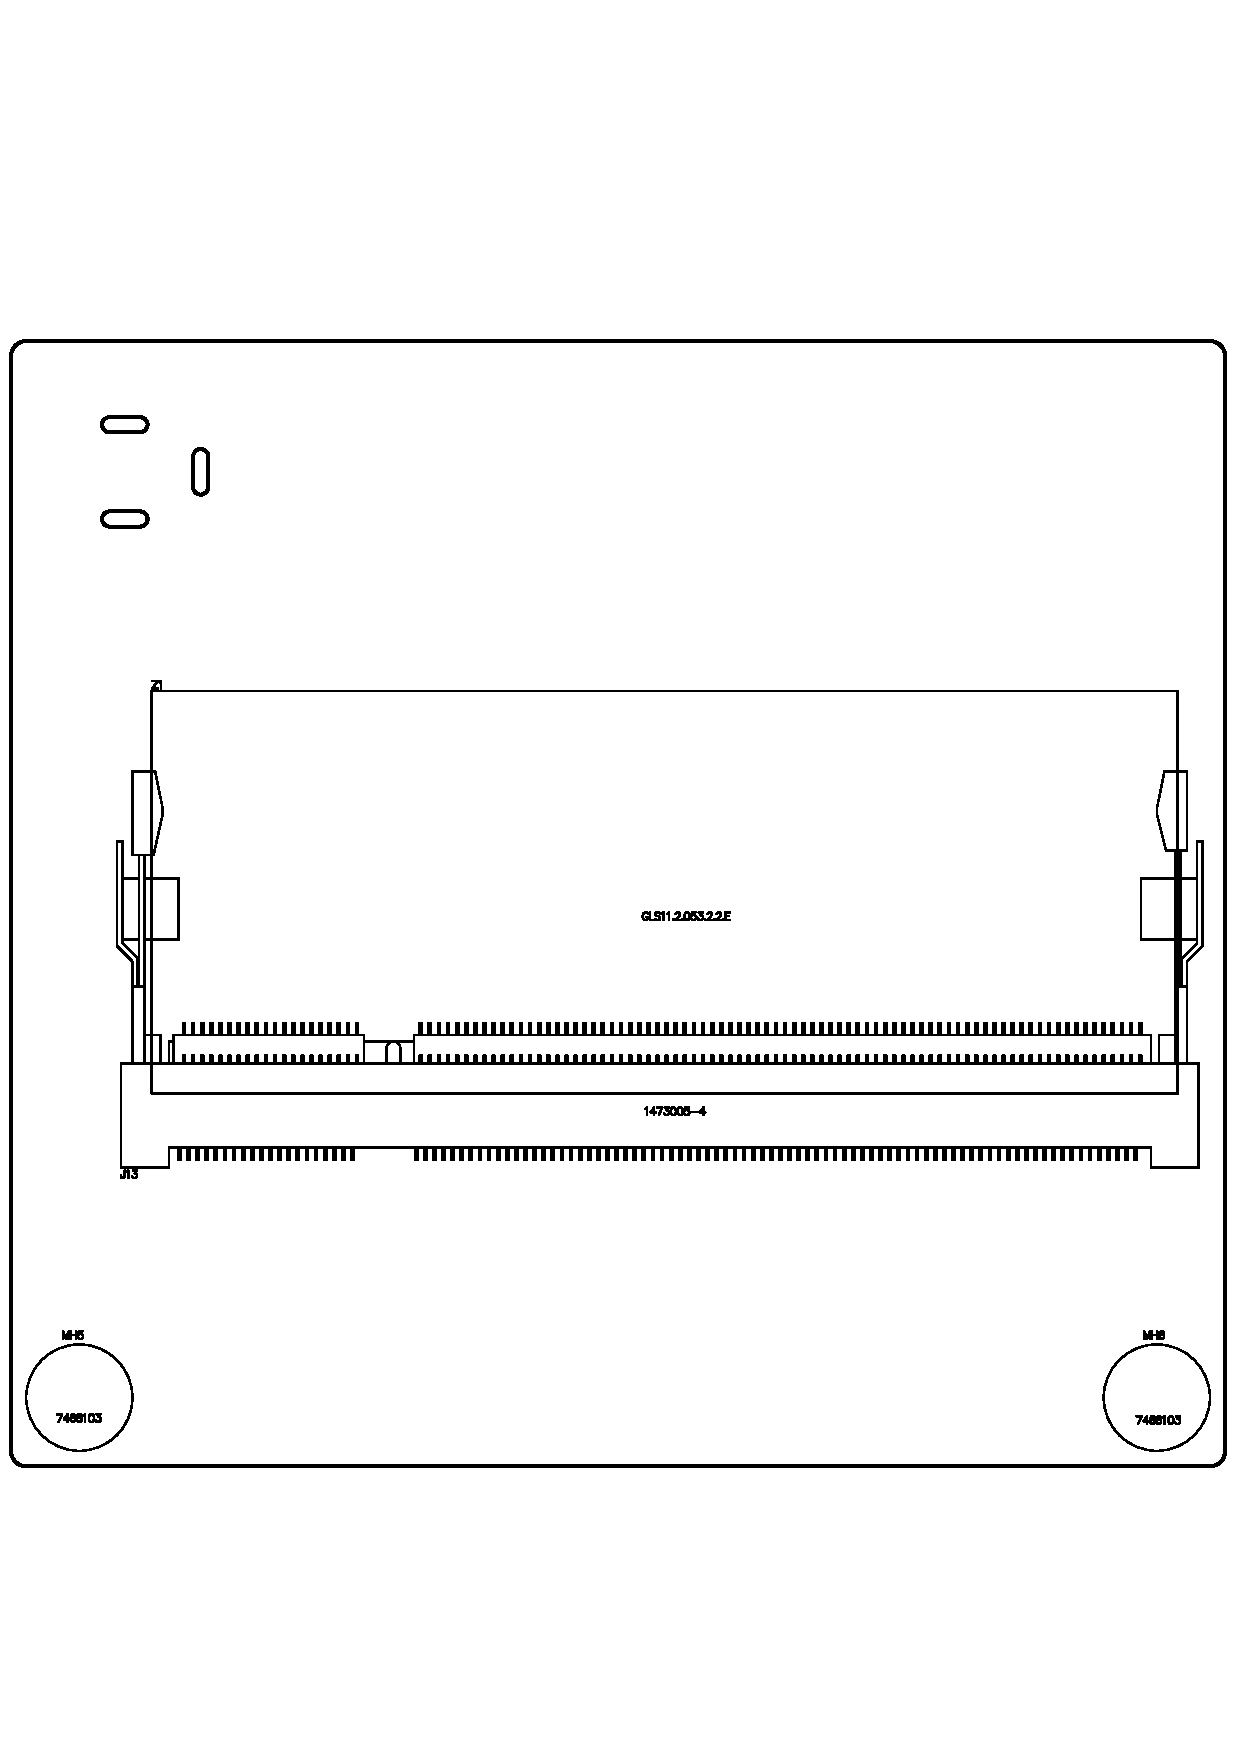
\includegraphics[width=0.9\linewidth,clip, trim=0cm 4cm 0cm 4cm]{./chapters/chapter5/liteboard_B.pdf}
		\caption{Strona B}\label{chilli:StronaB}
	\end{minipage}
\end{figure}


\section{Chiliboard}

Chiliboard jest to komputer jednopłytkowy (Single Board Computer) oparty na module chilliSOM~\cite{chiliboard}. Projekt ten posiada elementy elektroniczne i mechaniczne po obu stronach laminatu. Do procedury badań wybrano wersję Premium.

\breakparagraph{}
Ilość elementów elektronicznych: 140.

\begin{table}[H]
	\centering
	\caption{Poszczególne czasy na maszynach dla strony A}
	\begin{tabular}{lll}
		\toprule
		Nazwa maszyny                 & Czas operacji $[s]$ & Czas przezbrojenia $[s]$ \\
		\midrule
		stanowisko z sitodrukiem      & 10                  & 15                       \\
		automat pick\&place           & 435                 & 140                      \\
		ręczne układanie elementów & 15                  & 0                        \\
		lutowanie w piecu             & 300                 & 0                        \\
		lutowanie ręczne             & 85                  & 0                        \\
		kontrola wizualna             & 100                 & 0                        \\
		\bottomrule
	\end{tabular}
\end{table}

\begin{table}[H]
	\centering
	\caption{Poszczególne czasy na maszynach dla strony B}
	\begin{tabular}{lll}
		\toprule
		Nazwa maszyny                 & Czas operacji $[s]$ & Czas przezbrojenia $[s]$ \\
		\midrule
		stanowisko z sitodrukiem      & 10                  & 15                       \\
		automat pick\&place           & 0                   & 0                        \\
		ręczne układanie elementów & 10                  & 0                        \\
		lutowanie w piecu             & 100                 & 0                        \\
		lutowanie ręczne             & 0                   & 0                        \\
		kontrola wizualna             & 10                  & 0                        \\
		\bottomrule
	\end{tabular}
\end{table}

\begin{figure}[!htb]
	\begin{minipage}{0.5\textwidth}
		\centering
		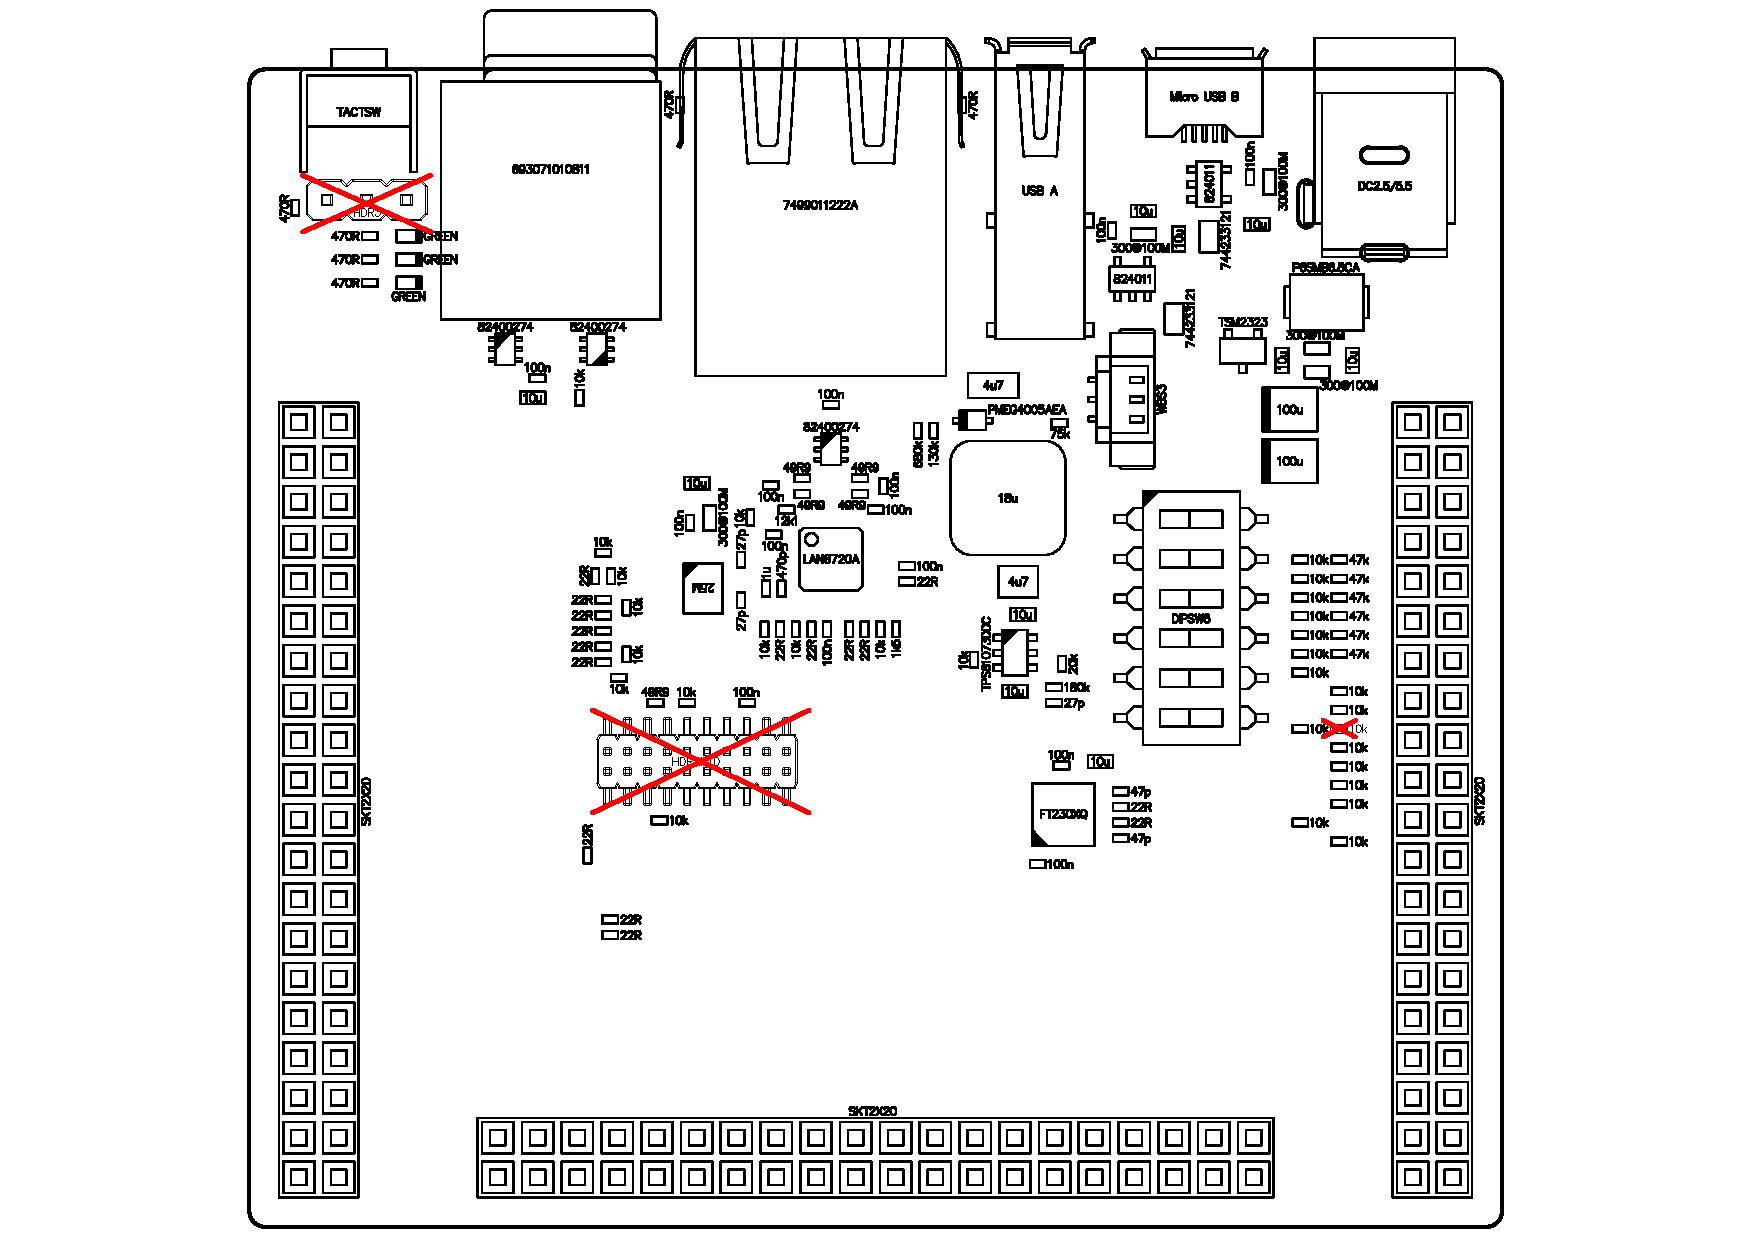
\includegraphics[width=\linewidth,clip, trim=3cm 0.2cm 3cm 0.1cm]{./chapters/chapter5/chilli_A.pdf}
		\caption{Strona A}\label{chilli:StronaA}
	\end{minipage}\hfill
	\begin{minipage}{0.5\textwidth}
		\centering
		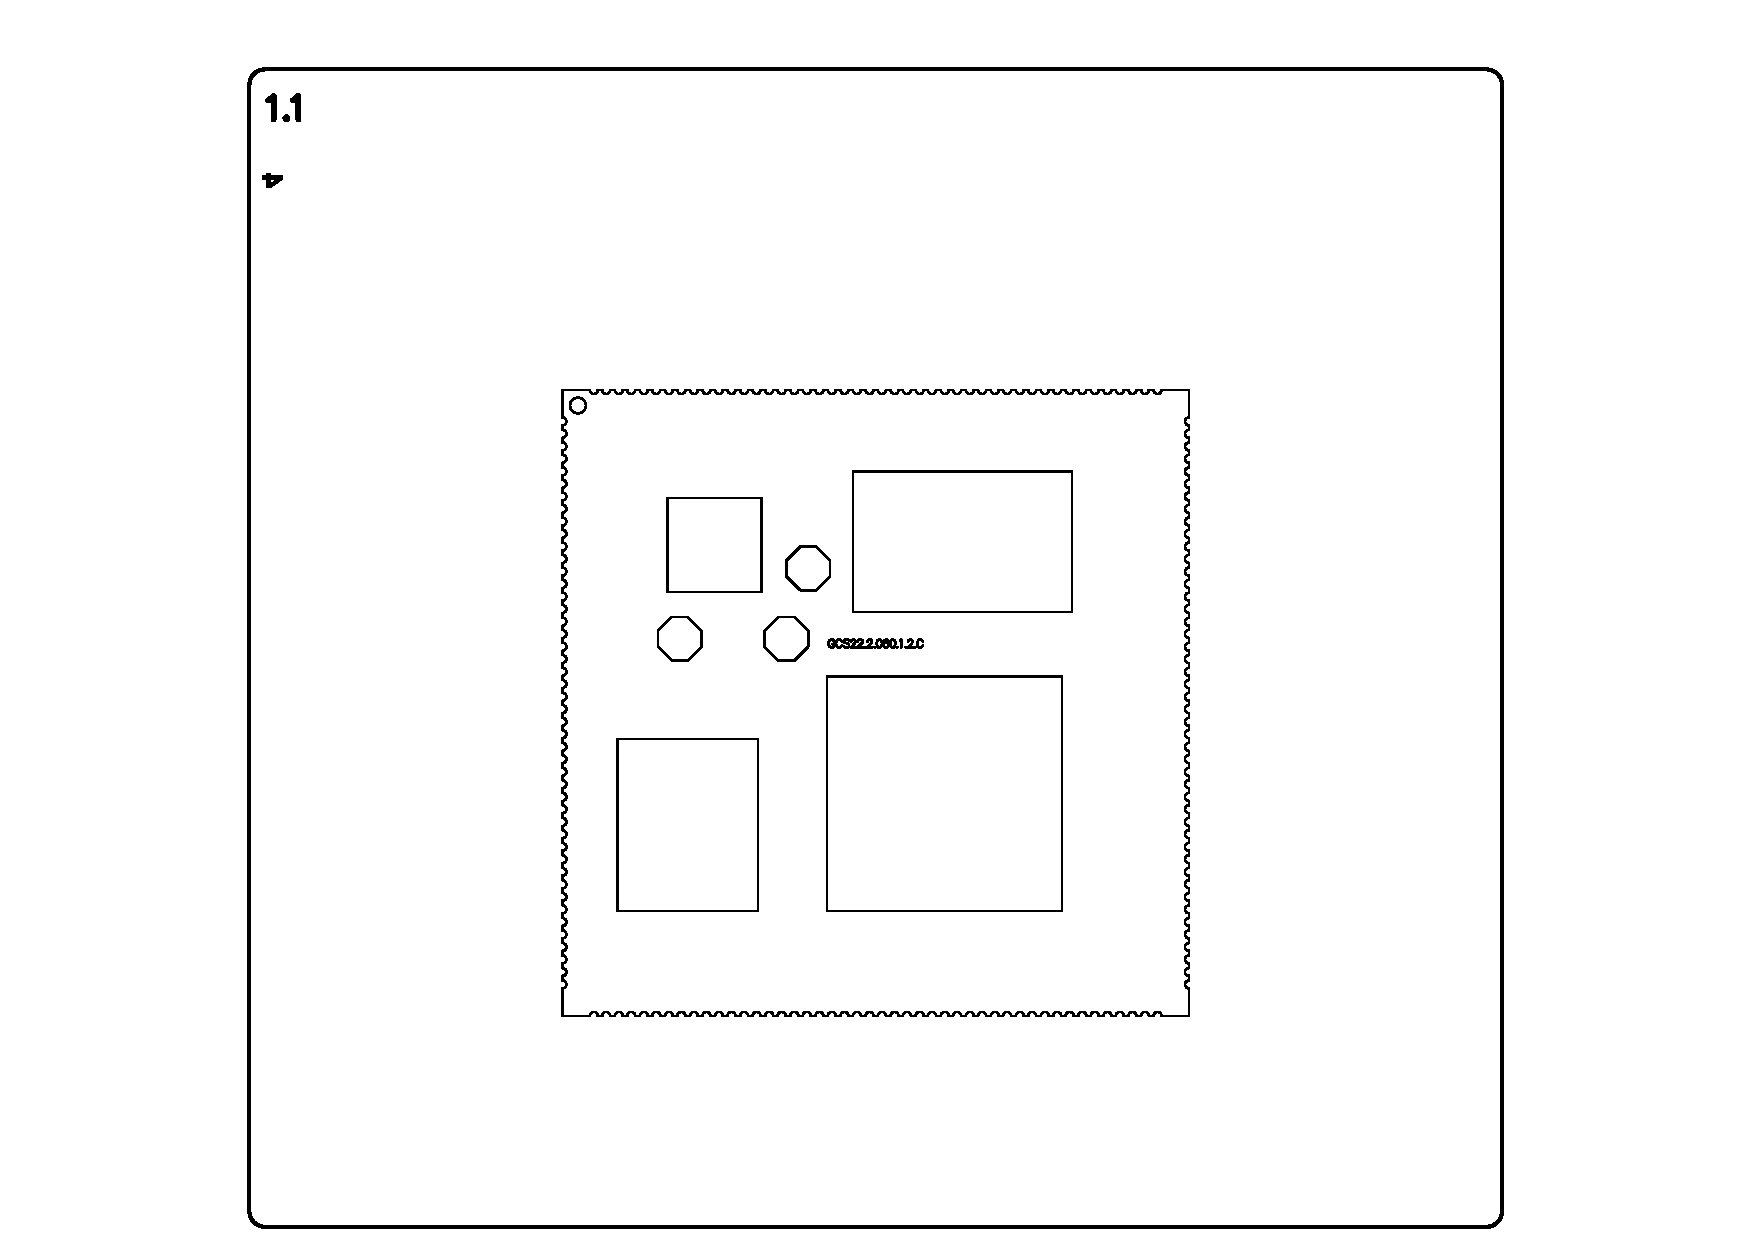
\includegraphics[width=\linewidth,clip, trim=3cm 0.1cm 3cm 0.1cm]{./chapters/chapter5/chilli_B.pdf}
		\caption{Strona B}\label{chilli:StronaB}
	\end{minipage}
\end{figure}

\section{Jetson Nano baseboard}
Przedsiębiorstwo NVIDIA udostępniło platformę Jetson Nano, która została wykorzystana przez Antmicro do stworzenia płyty protopowej (rozszerzeń).
Ten kompaktowy komputer jest ukierunkowany na całkowicie nowe aplikacje, takie jak tani monitoring wizyjny, czy roboty domowe z pełnymi możliwościami analitycznymi.
Dzięki temu, że kod źródłowy jest otwarty, może być ona dowolnie modyfikowana.

\breakparagraph{}
Ilość elementów elektronicznych: 232.

\begin{table}[H]
	\centering
	\caption{Poszczególne czasy na maszynach dla strony A}
	\begin{tabular}{lll}
		\toprule
		Nazwa maszyny                 & Czas operacji $[s]$ & Czas przezbrojenia $[s]$ \\
		\midrule
		stanowisko z sitodrukiem      & 10                  & 15                       \\
		automat pick\&place           & 643                 & 197                      \\
		ręczne układanie elementów & 50                  & 0                        \\
		lutowanie w piecu             & 260                 & 0                        \\
		lutowanie ręczne             & 190                 & 0                        \\
		kontrola wizualna             & 230                 & 0                        \\
		\bottomrule
	\end{tabular}
\end{table}

\begin{table}[H]
	\centering
	\caption{Poszczególne czasy na maszynach dla strony B}
	\begin{tabular}{lll}
		\toprule
		Nazwa maszyny                 & Czas operacji $[s]$ & Czas przezbrojenia $[s]$ \\
		\midrule
		stanowisko z sitodrukiem      & 10                  & 15                       \\
		automat pick\&place           & 107                 & 96                       \\
		ręczne układanie elementów & 0                   & 0                        \\
		lutowanie w piecu             & 260                 & 0                        \\
		lutowanie ręczne             & 0                   & 0                        \\
		kontrola wizualna             & 120                 & 0                        \\
		\bottomrule
	\end{tabular}
\end{table}

\begin{figure}[!htb]
	\begin{minipage}{0.5\textwidth}
		\centering
		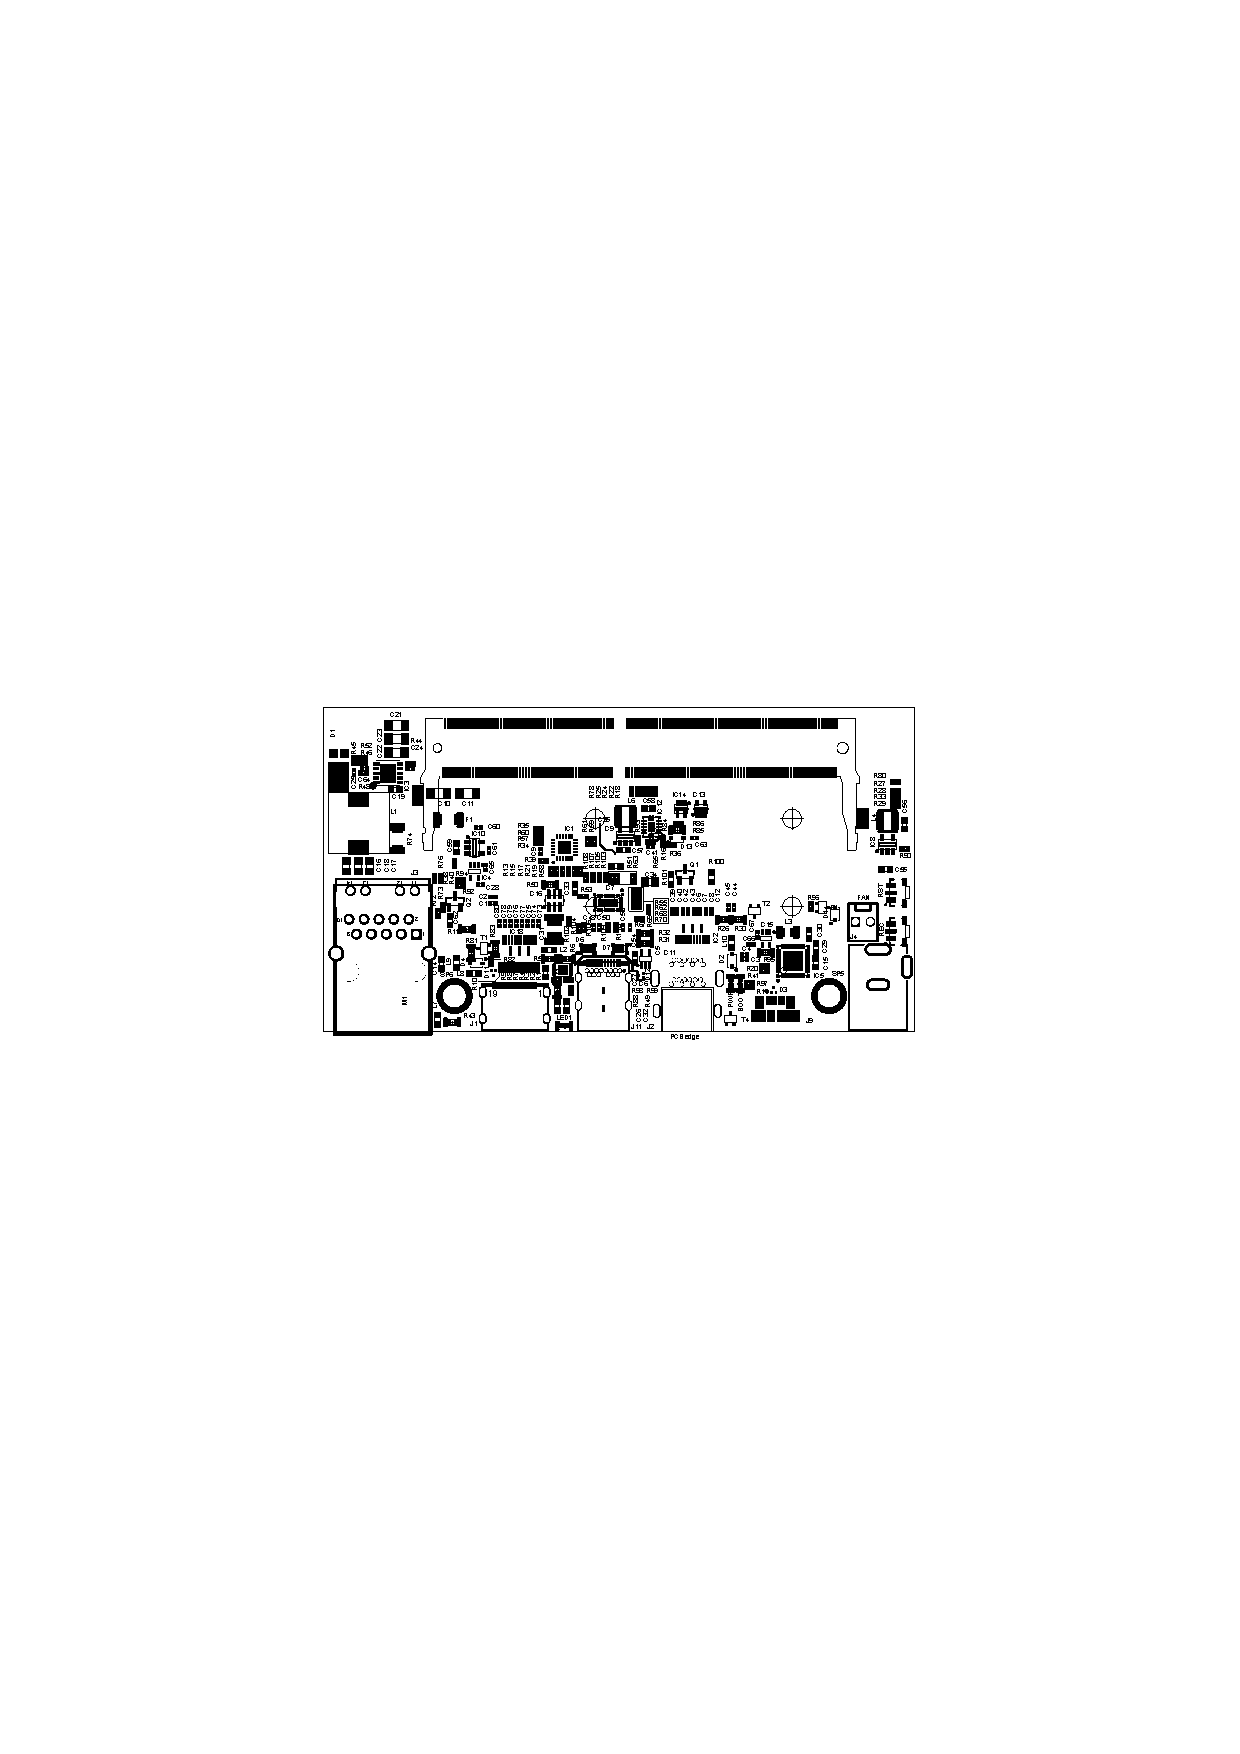
\includegraphics[width=0.95\linewidth,clip, trim=5.5cm 12cm 5.5cm 11cm]{./chapters/chapter5/Jetson_A.pdf}
		\caption{Strona A}\label{chilli:StronaA}
	\end{minipage}\hfill
	\begin{minipage}{0.5\textwidth}
		\centering
		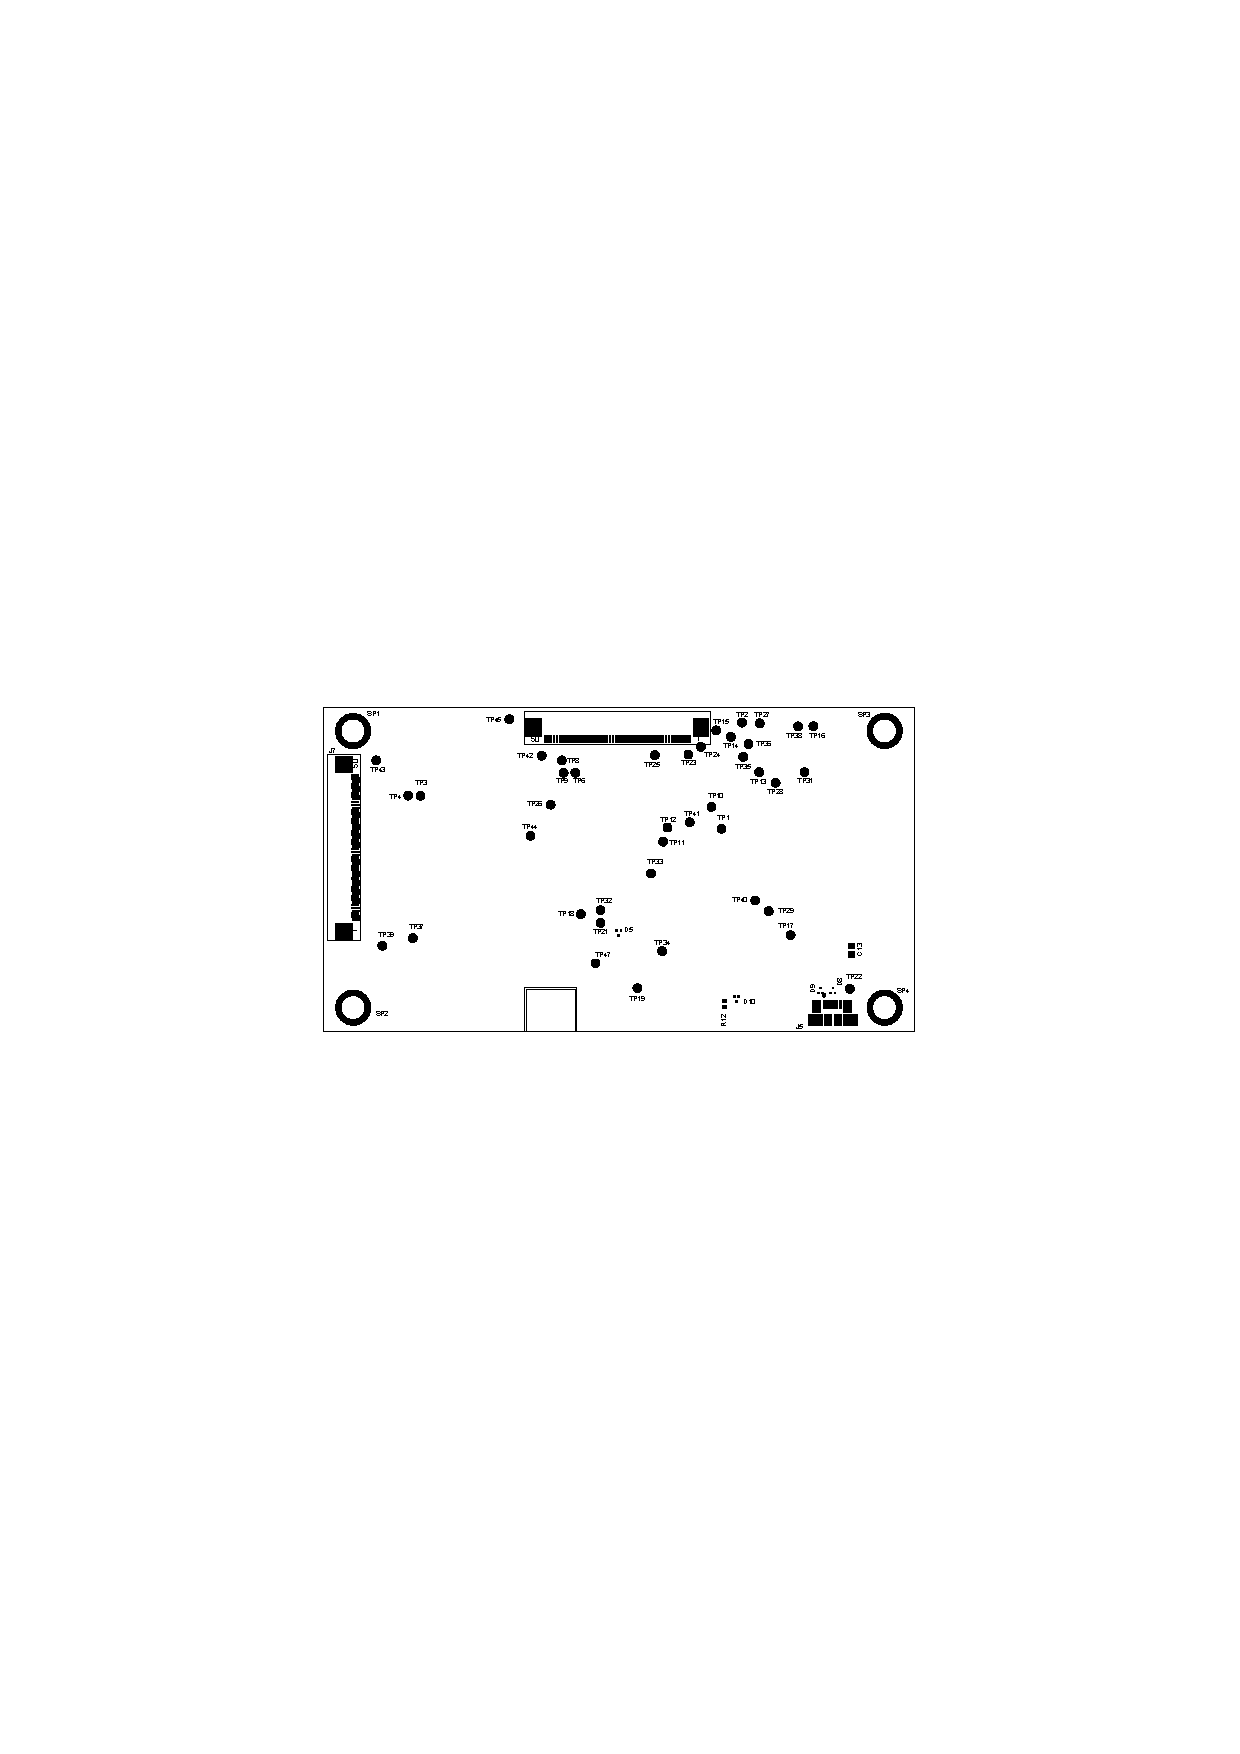
\includegraphics[width=0.95\linewidth,clip, trim=5.5cm 12cm 5.5cm 11cm]{./chapters/chapter5/Jetson_B.pdf}
		\caption{Strona B}\label{chilli:StronaB}
	\end{minipage}
\end{figure}

\section{KBox}
KBox to specjalistyczny system typu open-source, stworzone dla żeglarzy, aby umożliwić łączenie starych i nowych urządzeń na pokładzie. Stanowi świetne uzupełnienie komputera pokładowego. KBox jest zaprogramowany za pomocą platformy Arduino, a oprogramowanie wewnętrzne można łatwo skompilować na Windows, Mac i Linux.

\breakparagraph{}
Ilość elementów elektronicznych: 139.

\begin{table}[H]
	\centering
	\caption{Poszczególne czasy na maszynach}
	\begin{tabular}{lll}
		\toprule
		Nazwa maszyny                 & Czas operacji $[s]$ & Czas przezbrojenia $[s]$ \\
		\midrule
		stanowisko z sitodrukiem      & 10                  & 15                       \\
		automat pick\&place           & 390                 & 120                      \\
		ręczne układanie elementów & 30                  & 0                        \\
		lutowanie w piecu             & 300                 & 0                        \\
		lutowanie ręczne             & 85                  & 0                        \\
		kontrola wizualna             & 100                 & 0                        \\
		\bottomrule
	\end{tabular}
\end{table}

\begin{figure}[H]
	\centering
	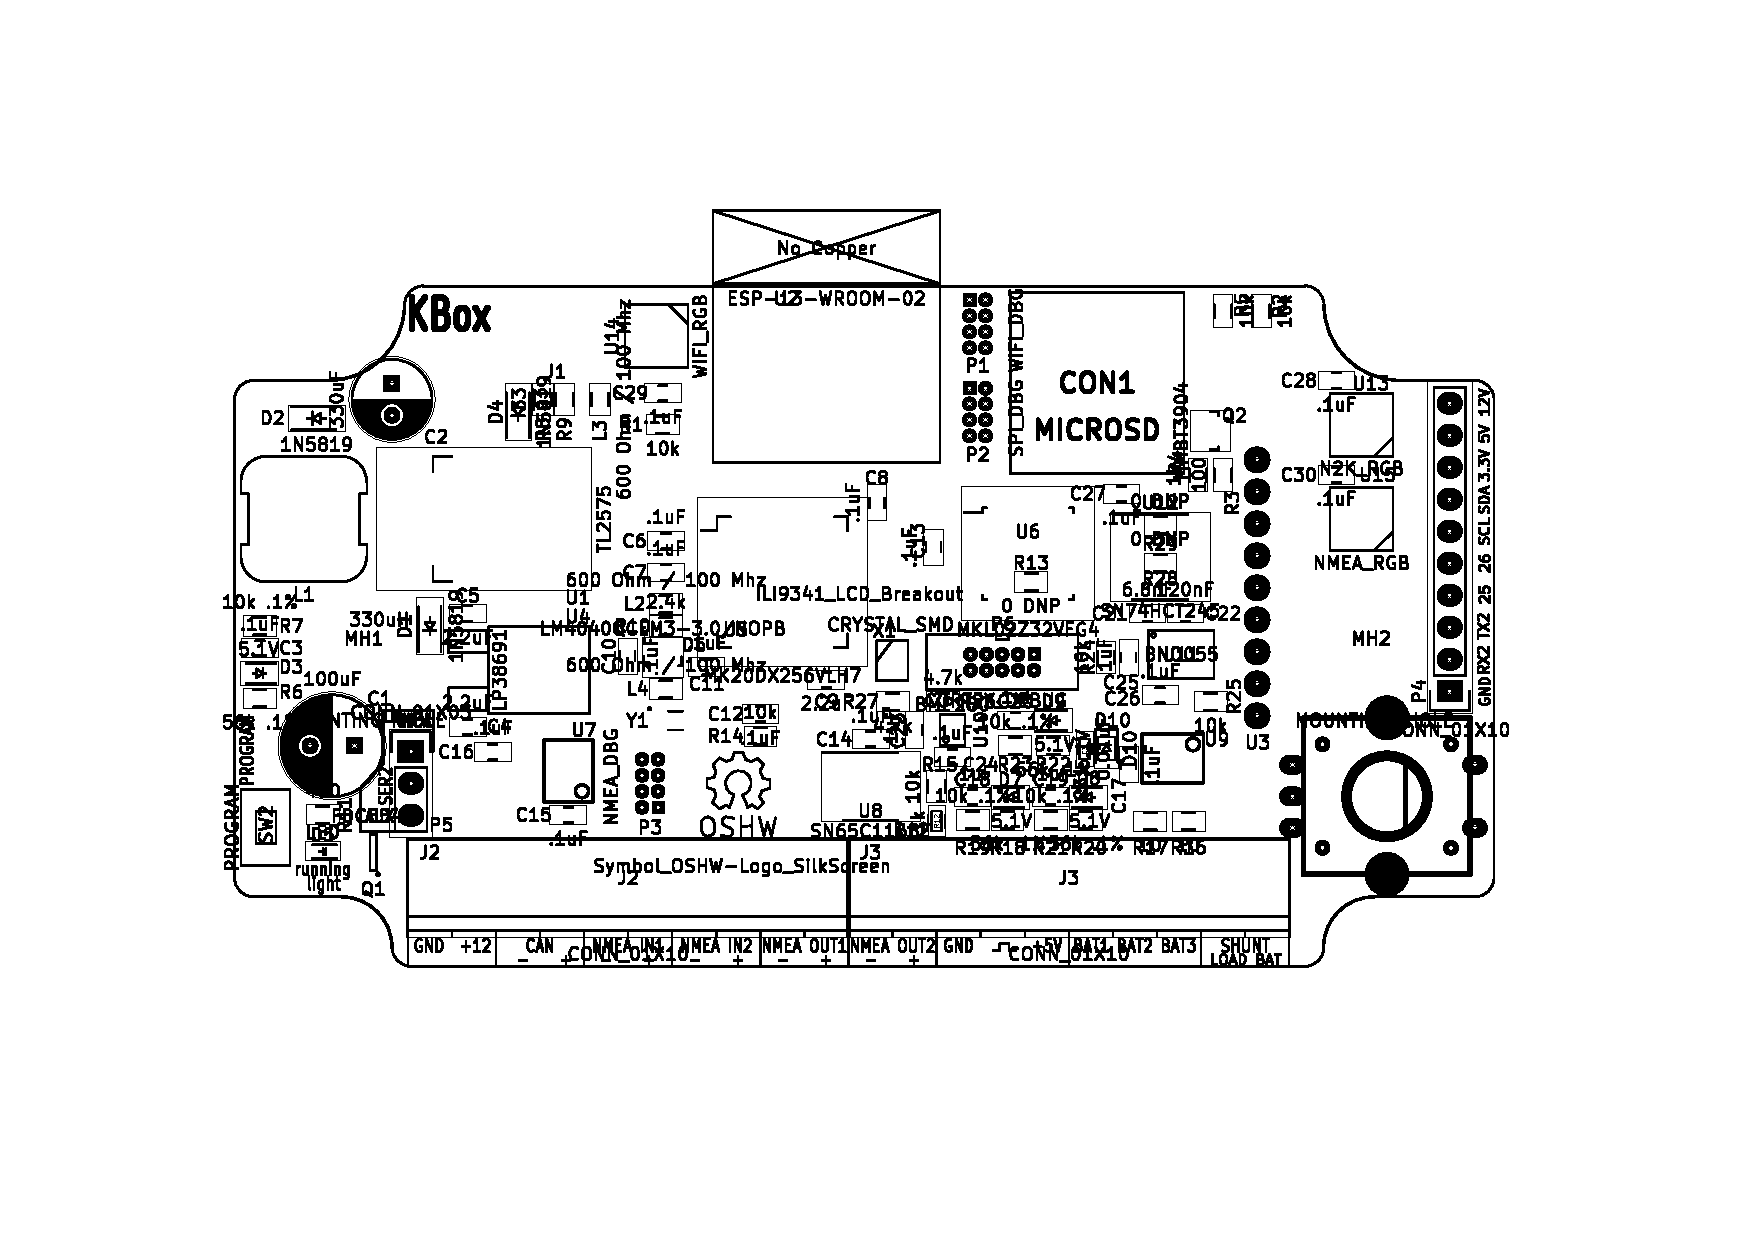
\includegraphics[scale=0.7,clip, trim=3.8cm 4cm 3.8cm 3cm]{chapters/chapter5/kbox-rotated.pdf}
	\caption{Schemat montażowy projektu KBox}
	\label{kbox}
\end{figure}

\newpage
\section{HackRF One}
HackRF One jest to urządzenie firmy Great Scott Gadgets, służące do odbioru i transmisji sygnałów radiowych. Ta platforma sprzętowa posiada licencję typu open-source (otwarte oprogramowanie) i może być stosowana jako peryferyjne urządzenie USB lub zaprogramowana do pracy samodzielnej.

\breakparagraph{}
Ilość elementów elektronicznych: 300.

\begin{table}[H]
	\centering
	\caption{Poszczególne czasy na maszynach}
	\begin{tabular}{lll}
		\toprule
		Nazwa maszyny                 & Czas operacji $[s]$ & Czas przezbrojenia $[s]$ \\
		\midrule
		stanowisko z sitodrukiem      & 10                  & 15                       \\
		automat pick\&place           & 760                 & 246                      \\
		ręczne układanie elementów & 0                   & 0                        \\
		lutowanie w piecu             & 260                 & 0                        \\
		lutowanie ręczne             & 210                 & 0                        \\
		kontrola wizualna             & 280                 & 0                        \\
		\bottomrule
	\end{tabular}
\end{table}

\begin{figure}[H]
	\centering
	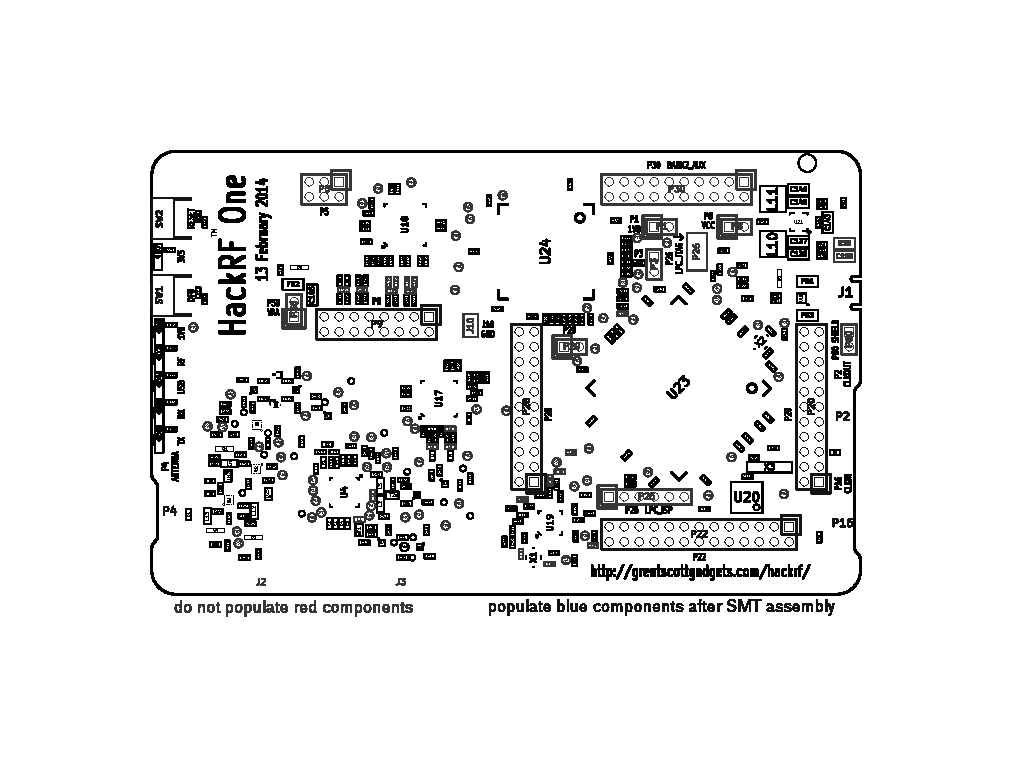
\includegraphics[scale=0.9,clip, trim=1.5cm 2.5cm 1.5cm 2.5cm]{chapters/chapter5/hackrf-one-assembly.pdf}
	\caption{Schemat montażowy projektu HackRF One}
	\label{hackrf}
\end{figure}

\newpage
\section{Wyniki badań}
Badania zostały przeprowadzone na komputerze PC z procesorem Intel Xeon E5--2673 v4 o taktowaniu 2.30GHz. Zbiór zadań posiadał 11 elementów i składał się on z projektów:
\begin{itemize}
	\item 2 x Liteboard
	\item 1 x Chiliboard
	\item 1 x Jetson Nano baseboard
	\item 1 x KBox
	\item 2 x HackRF One
\end{itemize}

Każde badania zostało przeprowadzone 4 razy. Czasy wykonywania się poszczególnych algorytmów zostały uśrednione.

Na początku zbadano wpływ temperatury początkowej na działanie algorytmu symulowanego wyżarzania (Tabela~\ref{tstart_sa}). Jak można zauważyć zwiększanie temperatury nie podniosło jakości otrzymanego rozwiązania. Efektem zmian jest tylko dłuższy czas wykonywania się algorytmu.

\begin{table}[H]
	\centering
	\label{tstart_sa}
	\caption{Wpływ $T_{start}$ gdy $T_{stop}=10$ i $\lambda=0.5$}
	\begin{tabular}{lll}
		\toprule
		                  & Czas wykonywania$[ms]$ & Moment zakończenia procesu$[s]$ \\
		\midrule
		$T_{start}=800$   & 6,19                   & 4503                             \\
		$T_{start}=8000$  & 7,78                   & 4503                             \\
		$T_{start}=80000$ & 10,15                  & 4503                             \\
		\bottomrule
	\end{tabular}
\end{table}

Kolejnym scenariuszem badanym jest zachowanie SA na różne wartości temperatury końcowej (Tabela~\ref{tstop_sa}). Zwiększanie tego parametru powoduję że program  szybciej kończy swoje działanie. Niestety ma to wpływ na skuteczności. Powodem tego jest że pod koniec procesu wyżarzania cząsteczki mają dużą ruchliwość (duże prawdopodobieństwo znalezienia gorszego rozwiązania).
\begin{table}[H]
	\centering
	\label{tstop_sa}
	\caption{Wpływ $T_{stop}$ gdy $T_{start}=8000$ i $\lambda=0.5$}
	\begin{tabular}{lll}
		\toprule
		                & Czas wykonywania$[ms]$ & Moment zakończenia procesu$[s]$ \\
		\midrule
		$T_{stop}=10$   & 5,82                   & 4503                             \\
		$T_{stop}=100$  & 2,07                   & 4503                             \\
		$T_{stop}=1000$ & 1,80                   & 4733                             \\
		\bottomrule
	\end{tabular}
\end{table}

\newpage
W ostatnim badaniu sprawdzono reakcję algorytmu na różne wartości $\lambda$ (Tabela~\ref{lamda_sa}). Parametr ten wpływa za szybkość spadku temperatury w SA\@. Im wartość niższa tym algorytm potrzębuję mniejszej ilości iteracji do zakończenia działania.
Według badań zbyt niska $\lambda$ powoduje że w symulowanym wyżarzaniu funkcja celu zbyt szybko zbiega do minimum lokalnego.
Odpowiednie dobranie wartości gwarantuje znalezienie lepszego rozwiązania ($\lambda = 0.5$) bez zbędnego wydłużania czasu działania algorytmu.

\begin{table}[H]
	\centering
	\caption{Wpływ $\lambda$ gdy $T_{start}=8000$ i $T_{stop}=10$}
	\label{lamda_sa}
	\begin{tabular}{lll}
		\toprule
		              & Czas wykonywania$[ms]$ & Moment zakończenia procesu$[s]$ \\
		\midrule
		$\lambda=0.2$ & 2,89                   & 4733                             \\
		$\lambda=0.5$ & 5,87                   & 4503                             \\
		$\lambda=0.8$ & 17,69                  & 4503                             \\
		\bottomrule
	\end{tabular}
\end{table}

W celu porównania skuteczności SA wykonano badania z użyciem algorytmu dokładnego. Przegląd zupełny znalazł optymalne rozwiązanie niestety kosztem długie czasu działania. POwodem tego jest złożoność obliczeniowa algorytmu która wynosi $11! = 39916800$ dla zbioru zadań jedenasto elementowego. Algorytm metaheurystyczny jest blisko 1069840 razy szybszy generując nieznacznie gorsze rozwiązanie.

\breakparagraph{}
Parametry symulowanego wyżarzania:
\\$T_{start}=8000$\\$T_{stop}=10$\\$\lambda=0.5$

\begin{table}[H]
	\centering
	\caption{Porównanie SA z przeglądem zupełnym}
	\label{comapte_sa_bf}
	\begin{tabular}{lll}
		\toprule
		                       & Czas wykonywania$[ms]$ & Moment zakończenia procesu$[s]$ \\
		\midrule
		Przegląd zupełny     & 6229699,69             & 4483                             \\
		Symulowane wyżarzanie & 5,82                   & 4503                             \\
		\bottomrule
	\end{tabular}
\end{table}